\chapter{Background}\label{C:related}

\section{Tracing}

There were two considered tracing frameworks to use. Implementation details of these frameworks are further discussed in Section \ref{C:workdone}.

The first framework considered was AspectJ. AspectJ uses byte code weaving to achieve the ability to trace method executions; this is when a piece of code is added to existing code without modifying the code itself and can be achieved through several different ways.

\begin{itemize}
\item Compile time:
The classes are compiled with the aspect weaved into them. When the jar is executed, the methods have the byte code from the aspect weaved into it already. This requires the source to be executed with AspectJ's compiler.
\item Load time:
This involves binary weaving deferred until the point in which a class loader will attempt to load in a class file. Achieved by using command line argument notifying java to use the AspectJ class loader.
\end{itemize}

AspectJ uses a point cut to identify what code is weaved and where in the code \cite{aspectwiki}. 

The other framework is Java Debugging Interface (JDI). JDI is similar to using an observer pattern. The list of classes to observe are selected, when a method is called the listening class will be notified if it has registered to be observed and will be given the information of the method call. 

\section{Performance Evaluation}
\label{performanceEvalBG}
The purpose for evaluating a performance of a given application is to create an understanding of the typical performance. For this typical performance to be valid, it has to be rigorous in design and implementation. This involves taking into consider a variety of factors that will be examined in reference to research papers that explore the issues.

Andy Georges et al. \cite{georges2007statistically} and Steve Blackburn et al. \cite{blackburn2008wake} present issues and alternatives to the current java performance methodologies used in research papers. They note that in premier conferences, 16 of the 50 papers examined did not examine the methodology they used. This limits the validity of the results and creates a situation where the experiment can not be reproduced. One of the main issues identified is specifying singular numbers, without expressing what the number is referring to (average, median, best, worst), leading to potential misleading representation of the results. A set of parameters that are of interest are explored in the paper, these include, heap size, start up performance, number of virtual machine (VM) invocations and handling of garbage collection. An experiment should also take into consideration the environment that the tests are going to be executed on.
\begin{itemize}
\item Heap Size -- A change in heap size can impact the garbage collection process. The smaller the heap size, the more often the garbage collector is run.
\item Start Up Costs  -- The costs associated with starting the application up. This will always involve class loading and just in time (JIT) re(compilation), it can also involve reading from a database and setting the application up.
\item Number of VM invocations -- The number of application runs that a single VM will execute.
\item Garbage Collection -- The process in identifying and removing objects that are no longer referenced.
\item Environment -- The hardware that the application is being run on.
\end{itemize}

\section{Related Work}
\label{relatedworkRef}
Testing is a critical part to any software engineering process, not only to stop incidents stemming from the the product, but also partially related to the increase in popularity of agile methodologies \cite{chaos}. Many of these methodologies employ test driven development and continuous integration resulting in testing becoming more important throughout the development process. For these reasons there have been research papers that examine the different approaches that can be taken to identify redundant test cases and reduce the size of test suites \cite{wong1995effect, wong1999test, rothermel1998empirical, rothermel2002empirical,koochakzadeh2009test,zhang2011empirical,li2008static}.

It is unclear whether programmatically reducing a test suite's size is worth the trade off in the ability to locate bugs.  Wong et al. \cite{wong1995effect, wong1999test} found that test suite reduction does not severely impact fault detection capability. In contrast to this finding, Rothermel et al. \cite{rothermel1998empirical, rothermel2002empirical} found that test-suite reduction can severely impact the fault detection capability. The uncertainty created by these conflicting studies motivates our research to decouple the removal of tests from the framework and move the responsibility onto the developers. 

A popular technique used in detecting redundancy involves analysing the statement executions, known as coverage information. Maurer, Garousi and Koochakzadeh \cite{koochakzadeh2009test} attempt to answer the question, is coverage information enough to determine redundant test cases? They state a redundant test case as being one that does not improve a specific criteria. For example, in Figure \ref{fig:venndiagram} we see that according to the statement coverage data of test cases, T1 ... T5, T4 and T5 are fully redundant as T3 covers the statements that are executed by those tests. They looked at two other criteria, branch coverage and granularities. Granularity criteria involved splitting the tests into setup, exercise (execution), verify (assert) and lastly teardown then performing analysis over each section. They implemented two different metrics in which both used the criteria described above. The first metric examined each individual test with respect to every other test. It was calculated by measuring the percentage of a test case that is also a subset of the other test case. The second metric examined each test case with respect to every test suite as a whole. It was calculated by measuring the percentage of a test case that is covered by the test suite without the test in it. Comparing with manual inspection, they were able to determine the level of false positive and actual redundant tests. Of the redundant tests manually identified, the algorithm matched 95\% of those. However, of the tests that were manually identified as being non-redundant, 52\% of these were identified as being redundant by the algorithm. They concluded that coverage-based information is vulnerable in giving false-positives when identifying redundant test cases, suggesting common code paths as being a root cause. Statement coverage criteria gave a high rate of detection, but the implementation allowed for false positives to impact the results. 

\begin{figure}[h]
\begin{center}
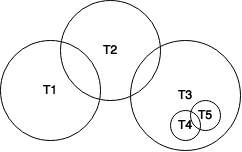
\includegraphics[]{VennDiagram.png}
\end{center}
\caption{The coverage of each test is shown by a circle. It shows that T4 and T5 are redundant as T3 already covers those statements.}
\label{fig:venndiagram}
\end{figure}

Zhang, Marinov, Zhang and Khurshid \cite{zhang2011empirical} examined the use of a greedy technique in comparison to heuristics. This required a criteria to be set by the tester, for example using statement coverage. The greedy technique would greedily select a test case that satisfies the maximum number of unsatisfied test requirements and would continue until all the test requirements had been satisfied. So the new test suite will contain exactly the same coverage as the old test suite while removing redundant test cases. This means that if a test subsumed another, then it would always be removed. The heuristic implementation was first conceived by Harrold, Gupta and Soffa \cite{harrold1993methodology} where essential test cases are selected as early as possible. Essential being that only one test case satisfies a test requirement exclusively. The heuristic approach resulted in the most cost-effective reduction, this being the amount of reduction and the fault-detection capability of the reduced test suites, showing that although greedy approach worked, there were better techniques available.

In situations where it is not possible to generate a spectrum to analyse, static analysis can be used to determine the level of redundancy. Robinson, Li and Francis \cite{li2008static} examine this. For the particular benchmark they use the test cases are written in a high level automation framework and consist of a list of commands. The commands perform actions such as file copying and loading configurations. To identify redundant test cases they examine the test cases commands as well as the instructions within the procedures that the test case loads. To calculate the similarities between two test cases, they consider three different metrics, Manhattan distance, unigram cosine similarity and bigram cosine similarity. They each were measuring how closely related two tests were based on the sequence of commands and procedures loaded. Their findings were similar to Maurer et al. \cite{koochakzadeh2009test} in that there are a large number of false - positives.

Static checking has several limitations in comparison to dynamic. Firstly, during run-time is when a large part of the paper trail is accessible. Before then the only information available is the method calls. \todo{Talk to Dave} Static checking therefore would provide useful information in a framework where dynamic data can not be collected and allows for the test cases to be examined in a static fashion such as the one used by Robinson, Li and Francis \cite{li2008static}. Dynamic allows for more data to be collected such as the parameters passed to a method as well as the ability to be executed on more suites. The papers examined looked at the coverage of a test suite at several different criterion levels but none looked at the spectra explicitly. This leaves a potentially useful approach to the problem that may help determine the level of redundancy within a test suite. 

When methods execute there is a trail of data that is left behind. Piecing together this data can show the relationships between methods, this relationship is known as a call graph. The call graph can be retrieved statically or dynamically \cite{graham1982gprof}. Static graphs represent every possible run of the program. Dynamic graphs represent one particular run. A static graph would require more information to be held and in the particular case of profiling test cases, dynamic would be more suitable due to the nature of a test case being the same for every run. A dynamic graph also allows for functional parameters to be collected. Xiaotong Zhuang and et al. \cite{Zhuang06accurate} describe a call tree as the overall tree of every method execution. To store the full call tree would involve an excess of memory, therefore they discuss the use of a calling context tree. This tree represents the same method executions however is compressed where the edge between the nodes contains a weighting, the weighting the number of occurrences of that method execution (calling frequency). Examining Figure \ref{fig:callgraph} shows the different variations that can be observed with the same data. The top left hand picture shows the method execution trail, where A calls B, then B calls D twice and A calls C, then C calls D once. The call graph image (top right) condenses the information into one node per method call. This method is the most condensed variation, but gives the least amount of information. Directly below this, (calling context tree) condense it slightly less. It separates each path into its own branch when it is unique to the tree, the connection between nodes contains a weighting which represent the frequency. Finally, the bottom left (call tree) creates a new path for every new method execution regardless of the uniqueness, giving us the most information about the context if the order is retained.

\begin{figure}[h]
\begin{center}
\includegraphics[width = \textwidth]{CallGraph.png}
\end{center}
\caption{A diagram showing the three different variations of Call Graph information. Where  each have a varying level of information that is stored.}
\label{fig:callgraph}
\end{figure}


Edit distance algorithms play an important part in many domains, ranging from signal processing to mutations in genome sequences \cite{navarro2001guided}. It calculates the number of edit operations needed to go from one string to another. There are a variety of different implementations of edit distance metrics. Cohen, Ravikumar and Fienberg \cite{cohen2003comparison} explore different edit distance metrics for name matching. They concluded that Monge and Elkan performed the best for string edit-distance metrics. The metric works by splitting the two strings into tokens, these tokens are then calculated to find the similarity using other common metrics such as Levenshtein distance. 

\todo{Describe the wilcoxin test here?}